% 
%  chapter3.tex
%  ISELthesis
%  
%  Created by Matilde Pós-de-Mina Pato on 2012/10/09.
%
\chapter{A Short \LaTeX~ Tutorial with Examples}
\label{cha:a_short_latex_tutorial_with_examples}

This Chapter aims at exemplifying how to do common stuff with \LaTeX. We also show some stuff which is not that common! ;) 

Please, use these examples as a starting point, but you should always consider using the \emph{Big Oracle} (aka, \href{http://www.google.com}{Google}, your best friend) to search for additional information or alternative ways for achieving similar results.


\section{Document Structure} % (fold)
\label{sec:document_structure}

In engineering and science, a thesis or dissertation is the culmination of a master's or Ph.D. degree. A thesis or dissertation presents the research that the student performed for that degree. From the student's perspective, the primary purpose of a thesis or dissertation is to persuade the student's committee that he or she has performed and communicated research worthy of the degree. In other words, the main purpose of the thesis or dissertation is to help the student secure the degree. 

From the perspective of the engineering and scientific community, the primary purpose is to document the student's research. Although much research from theses and dissertations is also communicated in journal articles, theses and dissertations stand as detailed documents that allow others to see what the work was and how it was performed. For that reason, theses and dissertations are often read by other graduate students, especially those working in the research group of the authoring student \cite{gustavii2016write, glasman2010science, chicago, strunk}. 
	
With a thesis or dissertation, the format also encompasses the names of the sections that are expected: 
\begin{enumerate}
\item Thesis Cover
\item Acknowledgments (if exist)
\item Abstract (Portuguese and English)
\item Index
\item List of Figures
\item List of Tables
\item Nomenclature/List of Abbreviations (if exists)
\item Glossary (if exists)
\item Introduction
\item State-of-the-Art or Related work
\item Proposed method
\item Experiment result
\item Conclusion and Future work
\item References, 
\item Gantt diagram (if exists), and 
\item Appendix (if exists)
\end{enumerate}
 
\subsection{State-of-the-Art}
\label{sec:state}

State-of-the-Art (SoTA) is a step to demonstrate the novelty of your research results. The importance of being the first to demonstrate research results is a cornerstone of the research business\footnote{``Why and how to write the state-of-the-art'', by Babak A. Farshchian, May 22, 2007}. 

Besides demonstrating the novelty of your research results, a SoTA has other important properties:
\begin{enumerate}
\item It teaches you a lot about your research problem. By reading literature related to your research problem you will learn from other researchers and it will be easier for you to understand and analyse your problem;
\item It proves that your research problem has relevance;
\item It shows different approaches to a solution;
\item It shows what you can reuse from what others have done. 
\end{enumerate}
 
 
\subsection{Related work}
\label{sec:relatedwork}

In the \textit{Related Works} section, you should discuss briefly about published matter that technically relates to your proposed work\footnote{\url{https://academia.stackexchange.com/questions/68164/how-to-write-a-related-work-section-in-computer-science}}.

A short summary of what you can include (but not limited to) in the Related Works section:
\begin{enumerate}
\item Work that proposes a different method to solve the same problem;
\item Work that uses the same proposed method to solve a different problem;
\item A method that is similar to your method that solves a relatively similar problem;
\item A discussion of a set of related problems that covers your problem domain.
\end{enumerate}
    

\section{Glossary and Nomenclature/List of Symbols} % (fold)
\label{sec:glossary}

Many technical documents use terms or acronyms unknown to the general population. It is common practice to add a glossary to make such documents more accessible. A \textit{glossary} is a nice thing to have in a report and usually very helpful. As you probably can imaging, it is very easy to create in \LaTeX. 

As with all packages, you need to load glossaries with \verb|\usepackage|, but there are certain packages that must be loaded before glossaries, if they are required: \texttt{hyperref, babel, polyglossia, inputenc} and \texttt{fontenc}.

\begin{verbatim}
\usepackage{glossaries} 
\makenoidxglossaries
\end{verbatim}

Once you have loaded \texttt{glossaries}, you need to define your terms in the preamble (or, separated file) and then you can use them throughout the document. 

Next you need to define the terms you want to appear in the glossary. Again, this must be done in the preamble. This is done using the command

\verb|\newglossaryentry{<label>}{<key-val list>}|

The first argument \verb|<label>| is a unique label to allow you to refer to this entry in your document text. The entry will only appear in the glossary if you have referred to it in the document using one of the commands listed later. The second argument is a comma separated \verb|<key>=<value>| list.

Inside the text you just need to use the command \verb|\gls{name}| or \verb|\glspl{name}| (plural name) to call it. For example, the following defines the term 'set' and assigns a brief description. The term is given the label set. This is the minimum amount of information you must give:

\begin{verbatim}
\newglossaryentry{set} % the label
{	name=set,            								% the term
 	description={a collection of objects} 	% a brief description
}
 \end{verbatim}

Other example, now the glossary associated with a symbol, \gls{U}:

\begin{verbatim}
\newglossaryentry{U}   % the label
{	name={universal set}, % the term
 	description={the set of all things} 		% a brief description
 	symbol={\ensuremath{\mathcal{U}}}  	% the associated symbol 
}
 \end{verbatim}
 
Here's a simple example:
\begin{verbatim}
\usepackage{glossaries} 
\newglossaryentry{ex}{name={sample},description={an example}}
\newacronym{svm}{SVM}{support vector machine}
\newacronym{beta}{$\beta$}{Second letter of the greek alphabet}
\newacronym{alpha}{$\alpha$}{First letter of the greek alphabet}

\begin{document}
Here's my \gls{ex} term. First use: \gls{svm}. 
Second use: \gls{svm}.

\textit{I want the \gls{beta} to be listed after the \gls{alpha}}.
\end{document}
\end{verbatim}

This produces: \textit{Here's my sample term. First use: support vector machine (SVM).\\ Second use: SVM.\\
I want the \gls{beta} to be listed after the \gls{alpha}.}

Do not use \verb|\gls| in chapter or section headings as it can have some unpleasant side-effects. Instead use \verb|\glsentrytext| for regular entries and one of \verb|\glsentryshort|, \verb|\glsentrylong| or \verb|\glsentryfull| for acronyms. Alternatively use glossaries-extra which provides special commands for use in section headings, such as \\ \verb|\glsfmtshort{<label>}|.

The plural of the word ``\gls{matrix}'' is ``matrices'' not ``matrixs'', so the term needs the plural form set explicitly:

 \begin{verbatim}
\newglossaryentry{matrix}% the label
{	name=matrix, % the term
 	description={a rectangular table of elements}, 
	plural=matrices % the plural
}
 \end{verbatim}

Given a set of numbers, there are elementary methods to compute its \acrlong{gcd}, which is abbreviated \acrshort{gcd}. This process is similar to that used for the \acrfull{lcm}.

\section{Importing Images} % (fold)
\label{sec:importing_images}

You can import external graphics using package \verb|graphicx|. You will find several examples here: \url{https://www.overleaf.com/learn/latex/Inserting_Images}. The most important command is \verb|\includegraphics|. \LaTeX ~itself treats the image like normal text, i.e. as a box of certain height and width. The package documentation list the options width and height, as well as others.

This syntax is fairly self-explanatory, however, one thing to note is the use of the \verb|\centering| command. There are other ways to center a figure, but this is the correct way to do it inside a float environment. You will almost always be using this command when using floats.
\begin{verbatim}
\begin{figure}[H]
\centering
\includegraphics[scale=1.5]{atom.png}
\end{figure}
\end{document}    
\end{verbatim}

% section importing_images (end)

\section{Floats Figures and Tables, and Captions} % (fold)
\label{sec:floats_figures_and_captions}

The tabular environment can be used to typeset tables with optional horizontal and vertical lines. \LaTeX~ determines the width of the columns automatically. The first line of the environment has the form: 
\verb|\begin{tabular}[pos]{table spec}|, where 
\begin{inparaenum}[(1)]
\item \verb|table spec|  tells \LaTeX~ the alignment to be used in each column and the vertical lines to insert; and, 
\item \verb|pos| can be used to specify the vertical position of the table relative to the baseline of the surrounding text. 
\end{inparaenum}
The number of columns does not need to be specified as it is inferred by looking at the number of arguments provided. It is also possible to add vertical lines between the columns here. You can draw beautiful tables with the \verb|booktabs| package \url{https://ctan.org/pkg/booktabs?lang=en}.

Some notes are important to followed, such as present in \tablename~ \ref{tab:results}: 
\begin{asparaenum}[i)]
	\item Not defined vertical lines;
	\item The legend must be on top;
	\item Use \verb|\toprule|, \verb|\midrule| and \verb|\bottomrule| to draw horizontal lines.
\end{asparaenum}
 
\begin{table}[ht]
	\caption{Table's rules.}
	\label{tab:results}
\centering
\begin{tabular}{llr}
\toprule
\multicolumn{2}{c}{Item} \\
\cmidrule(r){1-2}
Animal & Description & Price (\$) 
\\
\midrule
Gnat  & per gram & 13.65 \\
      & each     &  0.01 \\
Gnu   & stuffed  & 92.50 \\
Emu   & stuffed  & 33.33 \\
Armadillo & frozen & 8.99 \\
\bottomrule
\end{tabular}
\end{table}

\begin{sloppypar}
There are two ways to incorporate images into your \LaTeX~ document, and both use the graphicx package by means of putting the command  \verb|\usepackage{graphicx}|  near the top of the \LaTeX~ file, just after the documentclass command.
\end{sloppypar}

The two methods are

\begin{enumerate}
\item  include only PostScript images (esp. 'Encapsulated PostScript') if your goal is a PostScript document using dvips;
\item include only PDF, PNG, JPEG and GIF images if your goal is a PDF document using pdflatex, \texttt{TeXShop}, or other PDF-oriented compiler. 
\end{enumerate}

Some PNG images within my \LaTeX~ document. The quality of the image files is sufficient and the result using \LaTeX~ and viewing the resulting DVI file is quite looks good.

To get the best quality of the images in  PDF files I'd recommend using vector-based graphics for images. The best format to save images in is .pdf, see Figure \ref{fig:ra-vectorial}. With programs like \texttt{Inkscape}, you can draw as you would in MS Paint (and do much more), and because the images are vector-based instead of pixel-based, their quality should be preserved when converting to PDF in any way.    

In all cases, each image must be in an individual 1-image file; no animation files or multipage documents. 

There are two different ways to place two figures/tables side-by-side.  More complicated figures with multiple images. You can do this using subcaption environments\footnote{The subcaption package: \url{http://mirrors.ibiblio.org/CTAN/macros/latex/contrib/caption/subcaption.pdf}} inside a figure environment. Subcaption will alphabetically number your figures and you have access to the complete reference as usual through \verb|\ref{fig:figurelabel}|, \figurename~\ref{fig:figura-completa}, or \figurename~\ref{fig:ra-raster} using \verb|\ref{fig:subfigurelabel}|.

\begin{figure}[t!]
	\centering
    \begin{subcaptionblock}{.4\textwidth}
       \centering
       
\includegraphics[trim=0em 0 0 0, clip, width=\textwidth]{ra-vectorial}
       \caption{Vectorial}\label{fig:ra-vectorial}
     \end{subcaptionblock}%
     ~
     \begin{subcaptionblock}{.4\textwidth}
       \centering
       
\includegraphics[trim=0em 0 0 0, clip,width=\textwidth]{ra-raster}
       \caption{Raster}\label{fig:ra-raster}
     \end{subcaptionblock}%
  \caption{Subfigure example with vectorial and no-vectorial images}
  \label{fig:figura-completa}
\end{figure}

Using the package listings you can add non-formatted text as you would do with \verb|\begin{verbatim}| but its main aim is to include the source code of any programming language within your document. If you wish to include pseudocode or algorithms see \href{http://en.wikibooks.org/wiki/LaTeX/Algorithms_and_Pseudocode}{LaTeX/Algorithms\_ and\_Pseudocode}, as \lstlistingname ~\ref{lst:SetApp}.

%  \lstfromfile{language}{linerange}{caption}{label}{othersinsideoflstinoputlisting}{path}
% \lstfromfile{java}{59-64}{Static method - SetApp}{SetApp}{showlines=true,morekeywords={begin,System,out,print},numbers=left, firstnumber=59}{SetApp.java}

\begin{minipage}{\textwidth}
\lstset{language=R,numbers=left}
\begin{lstlisting}[
    %%frame=trBL,escapechar=|,
    caption={R-Code (Test).},
    label={code:test}
]
# comentário
square <- function(x) {
    x^2
    % |$x^{2}$|
}

# nerv
x <- c(1:100)
y <- square(x)
\end{lstlisting}
\end{minipage}
\section{Generating PDFs from \LaTeX~} % (fold)
\label{sec:generating_pdfs_from_latex}

\subsection{Generating PDFs with pdflatex} % (fold)
\label{ssec:generating_pdfs_with_pdflatex}

You may create PDF files either by using \verb|latex| to generate a DVI file, and then use one of the many DVI-2-PDF converters, such as \verb|dvipdfm|.

Alternatively, you may use \verb|pdflatex|, which will immediately generate a PDF with no intermediate DVI or PS files. In some systems, such as Apple, PDF is already the default format for \LaTeX~. I strongly recommend you to use this approach, unless you have a very good argument to go for \verb|latex| + \verb|dvipdfm|.

A typical pass for a document with figures, cross-references and a bibliography would be:
\begin{verbatim}
$ pdflatex template
$ bibtex template
$ pdflatex template (twice)
\end{verbatim}
\begin{sloppypar}
You will notice that there is a new PDF file in the working directory called \verb|template.pdf|. Simple :)
\end{sloppypar}


Please note that, to be sure all table of contents, cross-references and bibliography citations are up-to-date, you must run \verb|latex| once, then \verb|bibtex|, and then \verb|latex| twice.
% section generating_pdfs_with_pdflatex (end)

\subsection{Dealing with Images} % (fold)
\label{sub:dealing_with_images}

You may process the same source files with both \verb|latex| or \verb|pdflatex|. But, if your text include images, you must be careful. \verb|latex| and \verb|pdflatex| accept images in different (exclusive) formats.  For \verb|latex| you may use EPS ou PS figures. For \verb|pdflatex| you may use JPG, PNG or PDF figures.  I strongly recommend you to use PDF figures in vectorial format (do not use bitmap images unless you have no other choice).
% subsection dealing_with_images (end)


\subsection{Creating Source Files Compatible with both latex and pdflatex} % (fold)
\label{ssec:creating_source_files_compatible_with_both_latex_and_pdflatex}

Do not include the extension of the figure file file in the \verb|includegraphics| command, for instance use: 
\verb|\includegraphics{filename}|, and not: \verb|\includegraphics{filename.png}|.
In the first form, \verb|latex| or \verb|pdflatex| will add an appropriate file extension.

This means that, if you plan to use only \verb|pdflatex|, you need only to keep (preferably) a PDF version of all the images. If you plan to use also \verb|latex|, then you also need an EPS version of each image.\\
% subsection creating_source_files_compatible_with_both_latex_and_pdflatex (end)
% section generating_pdfs_from_latex (end)

{\Large To be included in the sections above} \\

If you are writing only one or two documents and aren't planning on writing more on the same subject for a long time, maybe you don't want to waste time creating a database of references you are never going to use. In this case you should consider using the basic and simple bibliography support that is embedded within \LaTeX~.

\LaTeX~ provides an environment called \texttt{thebibliography} that you have to use where you want the bibliography; that usually means at the very end of your document, just before the \verb|\end{document}| command. Here is a practical example:

\begin{verbatim}
\begin{thebibliography}{9}
\bibitem{lamport94}
  Leslie Lamport,
  \emph{\LaTeX: A Document Preparation System}.
  Addison Wesley, Massachusetts,
  2nd Edition,
  1994.
\end{thebibliography}
\end{verbatim}

In this document, the bibliography is in a separate document: \texttt{bi\-blio\-gra\-phy.bib}  where information is entered from \url{https://scholar.google.pt/}, as show  \figurename~\ref{fig:bibtex}.

\begin{figure}[ht]
	\centering
	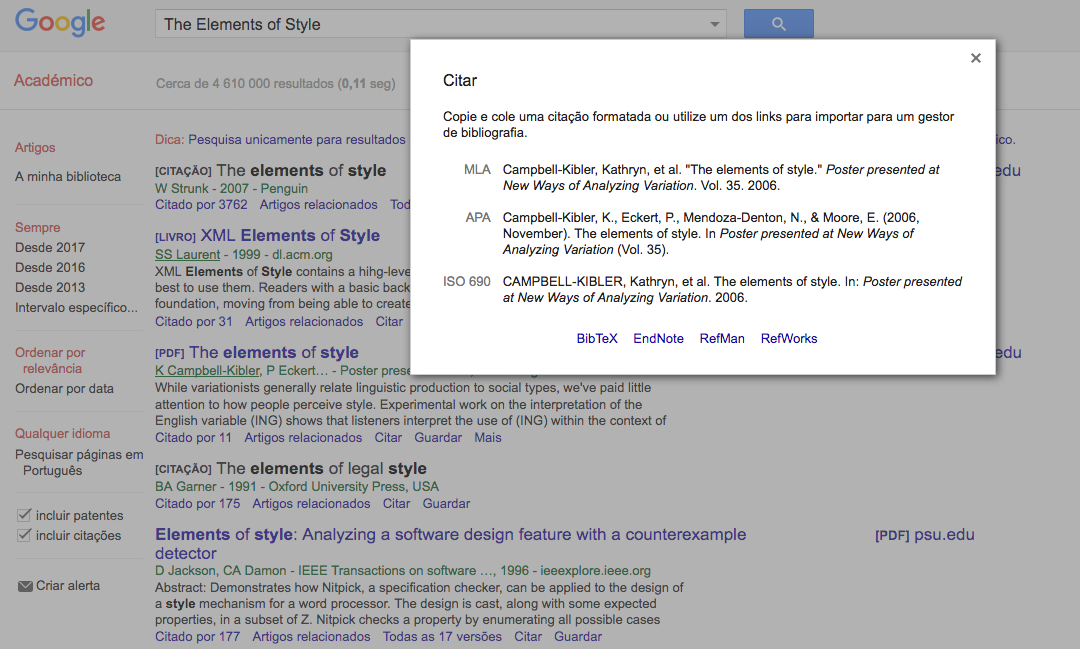
\includegraphics[width=0.85\textwidth]{bibtexexample}
	  \caption{Screenshot from Scholar Google}
  \label{fig:bibtex}
\end{figure}

To actually, cite a given document is \textit{very} easy. Go to the point where you want the citation to appear, and use the following: \verb|\cite{citekey}|, where the \texttt{citekey} is that of the \texttt{bibitem} you wish to cite, e.g \verb|~\cite{lamport94}|.  When \LaTeX~ processes the document, the citation will be cross-referenced with the bibitems and replaced with the appropriate number citation. The advantage here, once again, is that \LaTeX~ looks after the numbering for you.

When a sequence of multiple citations are needed, you should use a single \verb|\cite{}| command. The citations are then separated by commas. Note that you must not use spaces between the citations. Here's an result example \cite{strunk,chicago,texbook}.

Footnotes are a very useful way of providing extra information to the reader. Usually, it is non-essential information which can be placed at the bottom of the page. This keeps the main body of text concise.

The footnote facility is easy to use: \verb|\footnote{Simple footnote}|\footnote{Simple footnote}. 

\section{Equations}

Typesetting mathematics is one of \LaTeX's greatest strengths. It is also a large topic due to the existence of so much mathematical notation. It is recommend to read the following document available in \href{http://www.google.pt/url?sa=t&rct=j&q=&esrc=s&source=web&cd=1&cad=rja&ved=0CB4QFjAA&url=ftp%3A%2F%2Fftp.ams.org%2Fpub%2Ftex%2Fdoc%2Famsmath%2Fshort-math-guide.pdf&ei=DkScUOm8IJC5hAei7oGQDg&usg=AFQjCNEHl1pXuurNmXAdqfC0z-pPAbDyUw}{Short Math Guide for LaTeX - AMS - American Mathematical Society}.

\section{Page orientation}

\begin{sloppypar}
The default page layout is ``portrait'', but sometimes it is still useful/necessary to have the whole document or only single pages changed to ``landscape''. The latter might be due to a large table or figure. If you want to make appear the left side up, better readable on screen, the pdflscape-package will do it:
\verb|\usepackage{pdflscape}|
\end{sloppypar}
and again:
\begin{verbatim}
\begin{landscape}
...
\end{landscape}
\end{verbatim}

or, 
\verb|\includepdf[landscape=true,pages={1}]{example.pdf}|

to put the page in ``landscape'', while the rest will remain in ``portrait'' orientation. Nevertheless, the header/footer will also be changed in orientation.

\centering{\textbf{Written by Matilde Pós-de-Mina Pato with collaboration of Nuno Datia, \\2012 October (1st version)}}

% \centering{\textbf{Written by Matilde Pós-de-Mina Pato, \\ \today  \hspace{2em}--\version{2.6.2} (last version)}}
